\subsection*{GridSim simulates real scheduling scenarios} 
The experiments are conducted within the GridSim environment, which is modeled after a real power grid of a province of China.
The proportion of renewable generators in this test grid constitutes one-third of the total number of generators, and in certain scenarios, the maximum power generated by renewable units can surpass 60\% of the load. These align with the envisioned structure of future power systems with high penetration of renewable energy.


The core of GridSim is a professional power flow analysis program, solving power flow equations typically via the Newton-Raphson method\cite{wood2013power}. This professional program is widely employed in practical operations of the State Grid Corporation of China, enabling GridSim to boast sufficient physical fidelity to describe the complex state transitions of power systems. The provincial power grid, named SG-126, has 126 buses, 194 lines, 91 loads, and 54 generators, 17 of which are renewable. 


GridSim encompasses a whole year's operational snapshots, which enables RL agents to interact with the environment at any time of the year, thus facilitating the learning of robust and generalized scheduling policies.
These operational snapshots, which comprise load, renewable generation, and generators' power set-points, are derived from actual measurements. They were logged during a full year with data points spaced at 5-minute intervals, resulting in 105,120 operational snapshots. Additionally, the training and test datasets are separated, comprising measured snapshots of 2 consecutive years. This ensures that the agent learns generalized scheduling strategies and captures the essential dynamic characteristics of the grid operation instead of overfitting the training dataset. 


\subsection*{General scheduling capability demonstration}

\begin{figure}[h]
  \centering
  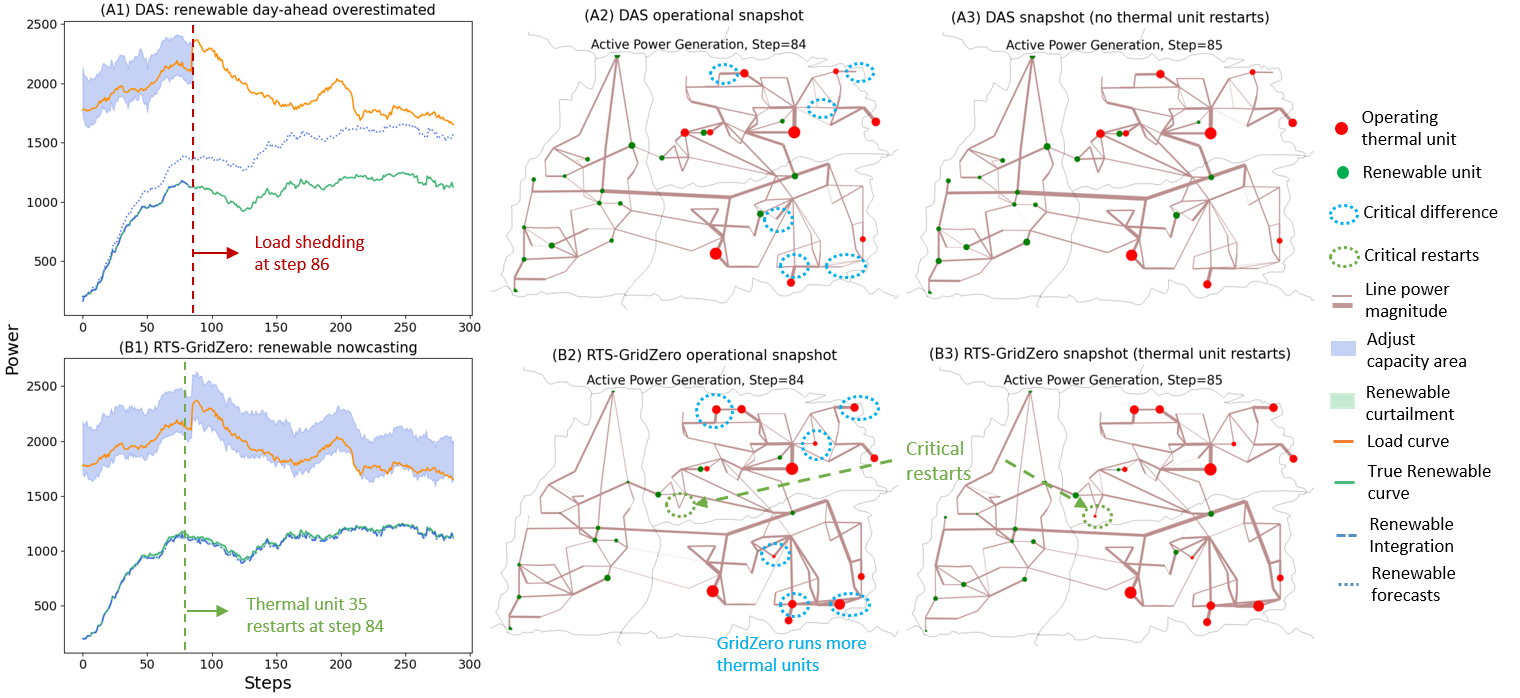
\includegraphics[width=1.0\linewidth]{fig/das_rts_snapshots.png}
  \caption{\textbf{RTS-GridZero reduces load shedding caused by renewable overestimation in the DAS framework.} Figures (A*) series indicate the performance of DAS under overestimated renewable forecasts, and figures (B*) series represent the performance of RTS-GridZero. 
  The red nodes indicate operating thermal units, and the green nodes represent operating renewable units. 
  The node sizes represent the magnitudes of active power generation. The line thicknesses represent the magnitudes of transmission power. The visualizations of grid operational snapshots are conducted in PYPSA~\cite{brown2017pypsa}. 
  As shown in (A1), DAS encounters a power mismatch when faced with a load surge at step 86. This is because that DAS relies on inaccurate day-ahead forecasts of renewable generation, leading to insufficient operating thermal units as marked by blue circles in (A2) and (B2). By using ultra-short-term forecasts and the ability to make look-ahead scheduling, GridZero first maintains a reasonable number of operating thermal units, which ensures sufficient ramping power if faced with load surges. Second, GridZero restarts thermal unit 35 at step 84, as marked by green circles in (B2) and (B3). These ensure that GridZero has adequate ramping power to handle the coming load surge at step 86.
  } 
  \label{fig:day_ahead_uc}
\end{figure}


\begin{figure}[h]
  \centering
  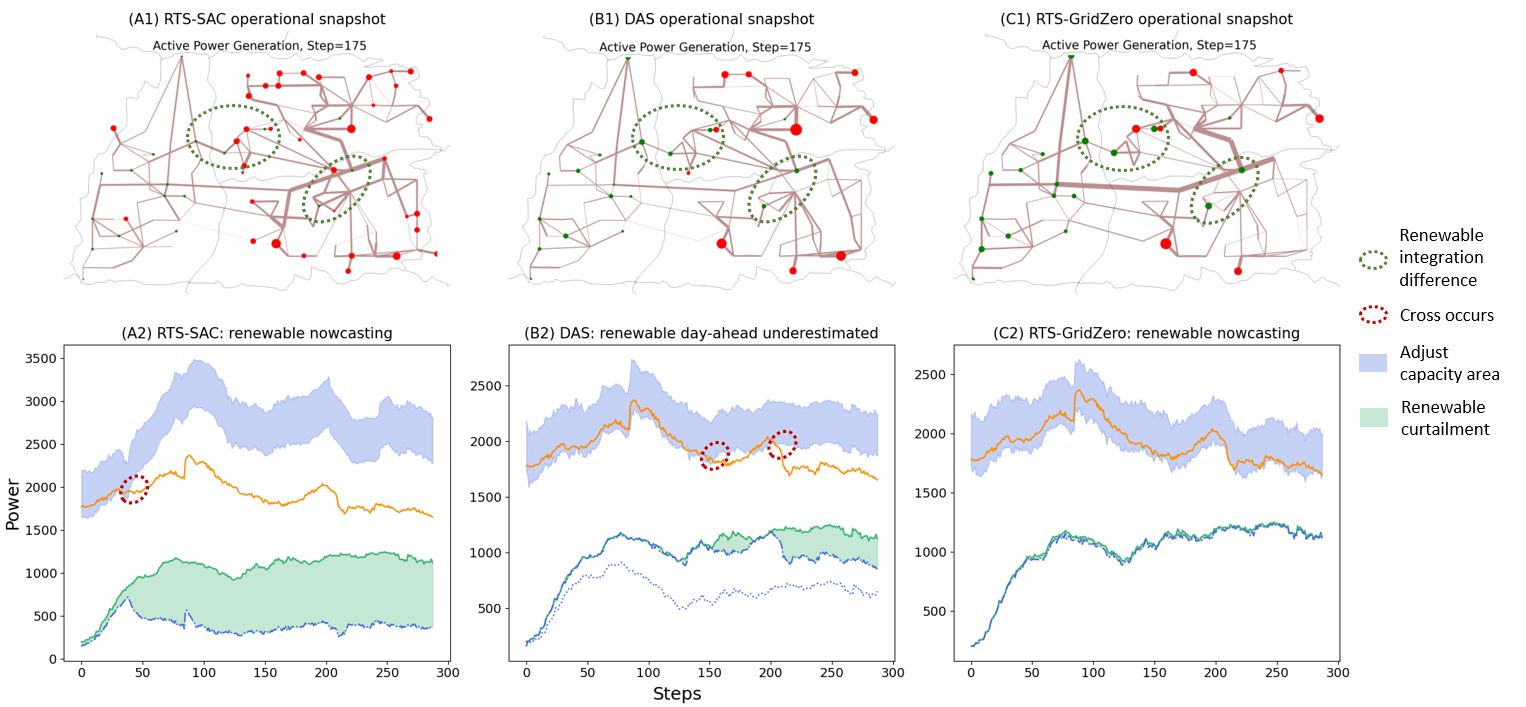
\includegraphics[width=1.0\linewidth]{fig/sac_das_gridzero.png}
  \caption{\textbf{RTS-GridZero outperforms SAC and DAS in reducing renewable curtailment.}
  SAC runs excessive thermal units leading to abundant renewable curtailment. DAS is also affected by underestimated renewable forecasts and maintains an excessive number of operating thermal units. These caused renewable curtailments since the lower bounds of the adjust capacity areas surpass the load curve, as marked by red circles in (A2) and (B2). With the powerful policy improvement and look-ahead scheduling brought by MCTS, GridZero learns efficient scheduling policies and integrates more renewable generation than SAC and DAS, as marked in green circles in (A1), (B1), and (C1). This significantly reduces renewable curtailment as shown in (C2). 
  } 
  \label{fig:renewable_curtailment}
\end{figure}
 

To evaluate the performance of GridZero, DAS, and SAC, a challenging test scenario is devised with a renewable generation proportion reaching up to 60\%. We choose SAC as the baseline of the model-free method because SAC performs better than DDPG and PPO in this scheduling problem.
The test scenario involves a whole-day scheduling task with 288 decision steps taken at 5-minute intervals. 
DAS is developed through the resolution of day-ahead unit commitment using the optimization software GUROBI and intraday economic dispatch using PYPOWER~\cite{lincoln2019pypower}. 
To demonstrate the advantages of our approach over traditional DAS, we first compare GridZero and DAS in reducing load shedding, as shown in Fig.\ref{fig:day_ahead_uc}. Second, we compare the performance of SAC, DAS, and GridZero in reducing the renewable curtailment, as demonstrated in Fig.\ref{fig:renewable_curtailment}.
SAC is also equipped with the proposed power balancing safety layer for effective exploration and is reproduced using the distributed APEX architecture which allows efficient data collection through multiple processes~\cite{horgan2018distributed}.


The DAS approach is prone to generating infeasible or suboptimal solutions if receiving inaccurate day-ahead forecasts, particularly in the UC problem.
If the renewable generation capacity is overestimated, as demonstrated in Fig.\ref{fig:day_ahead_uc}(A1), it can mislead DAS and result in insufficient operating thermal generators, as marked by blue circles in Fig.\ref{fig:day_ahead_uc}(A2). This is because that DAS's results are typically greedy, which makes it sensitive to prediction errors. The insufficient operating units caused a shortage in ramping power and a mismatch between generation and load power at step 86, as shown in Fig\ref{fig:day_ahead_uc}(A1). In real-world power grid operations, such power mismatches affect the frequency stability, leading to load shedding or even more serious consequences, such as grid collapse\cite{enwiki:1103904998}. However, GridZero solves this problem by look-ahead scheduling, it doesn't optimize the operational cost greedily but chooses the scheduling decision with a high expected return in the future, in which robustness has a greater impact. GridZero maintains a reasonable number of operating thermal units, as marked by blue circles in Fig.\ref{fig:day_ahead_uc}(B2). It anticipates the coming load surge in the look-ahead search process and restarts the thermal generator 35 at step 84 in advance, as marked by green circles in \ref{fig:day_ahead_uc}(B2) and (B3).

On the other hand, the underestimated renewable generation capacity also misleads DAS to run an excessive number of operating thermal generators, as shown in Fig.\ref{fig:renewable_curtailment}(B1). This causes the lower bound of the adjust capacity area to surpass the load consumption, as marked by red circles in Fig.\ref{fig:renewable_curtailment}(B2), resulting in the curtailment of renewable integration. This, in turn, increases carbon emissions and the costs of grid operations. 
The adjustment capacity area is based on the assumption of full integration of renewable generation.

Model-free RL methods, such as SAC, are commonly criticized for potentially inaccurate value estimations. This can cause instability in policy improvements and the scheduling agent is not able to integrate renewable generation reasonably, referred to as abundant renewable curtailment. As demonstrated in Fig.\ref{fig:renewable_curtailment}(A1) and (A2), SAC employs an excessive number of thermal generators starting from step 40, causing the adjustment capacity area to significantly surpass the load curve, as marked by the red circle in \ref{fig:renewable_curtailment}(A2). This in turn leads to a significant amount of renewable generation being curtailed.

However, with the utilization of ultra-short-term predictions and a well-designed look-ahead scheduling strategy, GridZero is able to make prompt and rational decisions regarding the power outputs of all generators and startup/shutdowns of thermal units, thereby ensuring that the adjustment capacity area aligns with the load consumption curve. This observably reduces renewable curtailment, as demonstrated in Fig.\ref{fig:renewable_curtailment}(C1) and (C2). 

\subsection*{Quantative analysis of GridZero and other methods}

\begin{table}[h]
\centering
\caption{Test statistics of GridZero, SAC, and traditional DAS (4 runs with 20 seeds). The RL-based RTS methods achieve much faster computation speed than the DAS precalculation framework by shifting the computation burden from the optimization process to an offline training phase. GridZero also much outperforms SAC in general performance and better observes operational constraints. $T_\text{episode}$ is 288-step decision-making time of a whole day. $\vert V_\text{bus}\vert$ is the voltage magnitude of the bus. $Q$ is the reactive power output of the generator.}
\begin{tabular}{cccc}
    \toprule
      & SAC & DAS & \textbf{GridZero} \\
    \midrule
    $T_{\text{episode}}$(s) & $21.2\pm{1.8}$ & $8557.3\pm{304.1}$ & $43.2\pm{2.1}$ \\
    Cumulative rewards & $256.8\pm{51.3}$ & 
    -
    & $\textbf{628.3}\pm{35.2}$ \\
    $\vert V_\text{bus}\vert$ violation(\%) & $0.3\pm{0.2}$ & $0.8\pm{0.1}$ & $0.5\pm{0.1}$ \\
    $Q$ violation(\%) & $15\pm{7}$ & $10\pm{1}$ & $\textbf{6.5}\pm{2}$ \\
    $P_{\text{balanced}}$ violation(\%) & $0.2\pm{0.3}$ & $0\pm{0.1}$ & $\textbf{0.05}\pm{0.05}$ \\
    Line soft overflow(\%) & $6\pm{4}$ & $8.8\pm{0.3}$ & $\textbf{3}\pm{3}$ \\
    Line hard overflow(\%) & $0.5\pm{0.1}$ & $0.1\pm{0.1}$ & $\textbf{0}\pm{0.01}$ \\
    Operating cost & $51135\pm{4000}$ & $41237\pm{200}$ & $\textbf{39785}\pm{2500}$ \\
    Renewable consumption(\%) & $55\pm{5}$ & $89\pm{0.5}$ & $\textbf{95}\pm{2}$\\
    \bottomrule
  \end{tabular}
  \label{tab:statitics}
\end{table}


\begin{figure}[h]
  \centering
  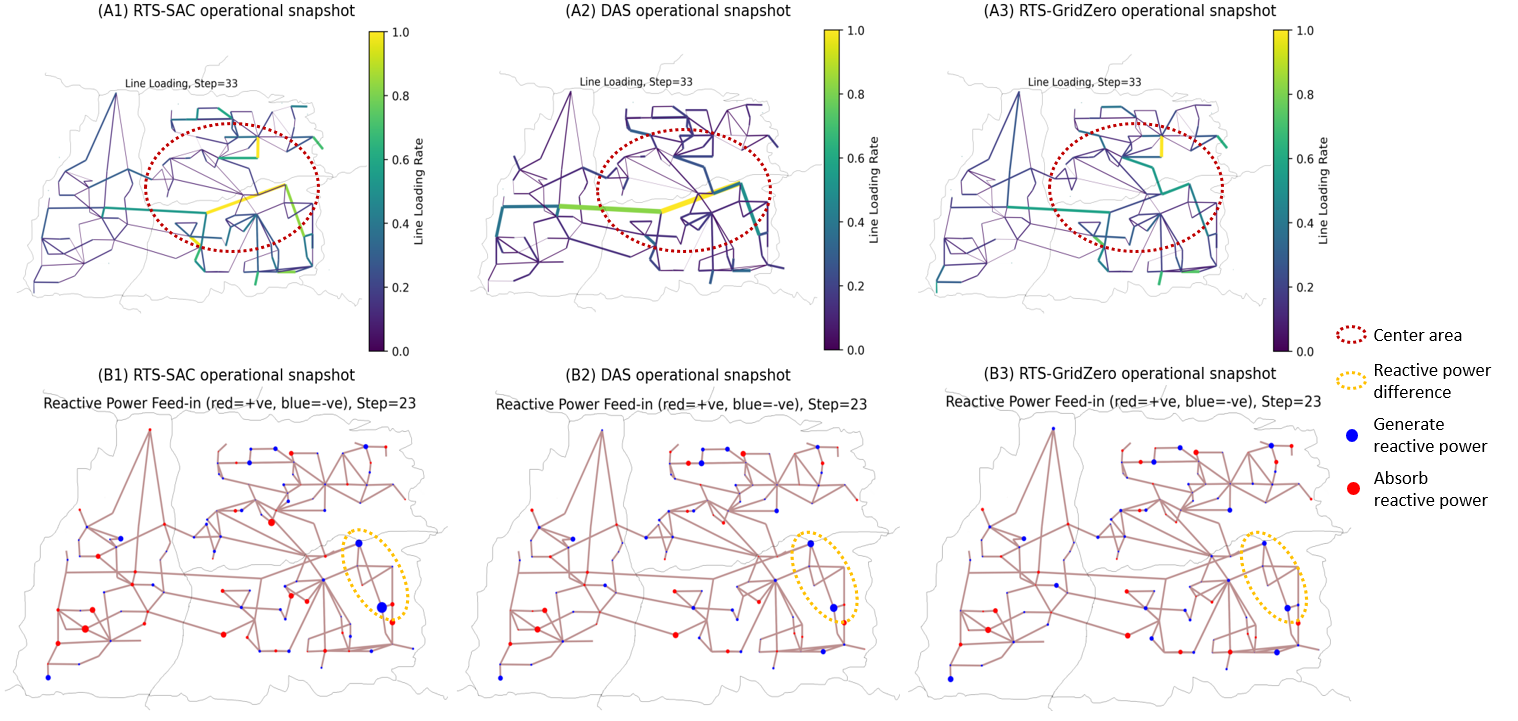
\includegraphics[width=1.0\linewidth]{fig/sac_das_gridzero_line_reactive.png}
  \caption{\textbf{Visualizations of line loading and reactive power dispatching.}
  Figures (A*) series indicate the operational snapshots of line loading, and figures (B*) series represent the operational snapshots of reactive power. For line loading, a reasonable strategy is to balance the load rate of each line and to avoid the situation that line loading is heavy. As marked by red circles in (A1), (A2), and (A3), GridZero achieves more average line loading than DAS and SAC in the center area. For reactive power, a reasonable strategy is to avoid reactive power converging on a small number of buses, which might lead to reactive power out-of-limit. GridZero also alleviates the reactive power convergence as marked by yellow circles in (B1), (B2), and (B3). The red nodes absorb reactive power and the blue nodes generate reactive power. 
  } 
  \label{fig:overflow_reactive}
\end{figure}

In addition to superior performance in representative scenarios, GridZero outperforms both DAS and SAC in various scheduling quality metrics.
As shown in Table.\ref{tab:statitics}, our method achieves 188.9 times faster than the conventional DAS method, corresponding to 0.15 seconds per decision step, which ensures the ability of real-time scheduling. DAS solves a mixed integer programming problem with 10080 discrete variables and 15552 continuous variables in a whole-day scheduling task, which is highly time-intensive. GridZero also outperforms SAC and DAS in terms of constraints and operating costs. 
The score of DAS is not shown because DAS is not capable of making single-step decisions like RL agents in GridSim. 
Our approach leverages ultra-short-term forecasts to make instant adjustments to generators, providing greater flexibility than traditional methods that rely solely on day-ahead plans. This allows the grid to make better use of renewable energy sources and minimize power generation costs.

The line loading is visualized in Fig.\ref{fig:overflow_reactive}(A*). GridZero maintains more average line loading, which could help reduce transmission overflows and line outages. In Fig.\ref{fig:overflow_reactive}(B*), GridZero also achieves more balanced reactive power dispatch and avoids reactive power convergence in Fig.\ref{fig:overflow_reactive}(B1). This can help reduce the violations of generator reactive power limits.



\subsection*{GridZero reduces the cost of flexibility retrofits and energy storage}
Real grid simulation results show that GridZero is able to achieve efficient real-time scheduling without the need for additional flexible resources, resulting in lower levels of renewable curtailment and load shedding. On the other hand, maintaining the DAS framework without changes necessitates significant hardware upgrades to enhance the grid's flexible resources. Such hardware improvements often require substantial investments.
 
More specifically, the hardware upgrades required for the DAS framework to reduce renewable curtailment and load shedding can be divided into two main directions, namely thermal units' flexibility retrofit and energy storage construction.
The objective of thermal units' flexibility retrofit is to lower the minimum operating power of thermal generators. 
In this way, even if the renewable energy power generation is underestimated, resulting in excessive thermal power generators operating, the output power of thermal generators can be reduced sufficiently to avoid renewable energy curtailment.
Energy storage serves a similar purpose, reducing the mismatch between renewable energy and load by storing excess renewable power during off-peak periods and releasing the stored electricity when the power supply is tight.
Both these directions involve significant investments. 


\begin{figure}[h]
  \centering
  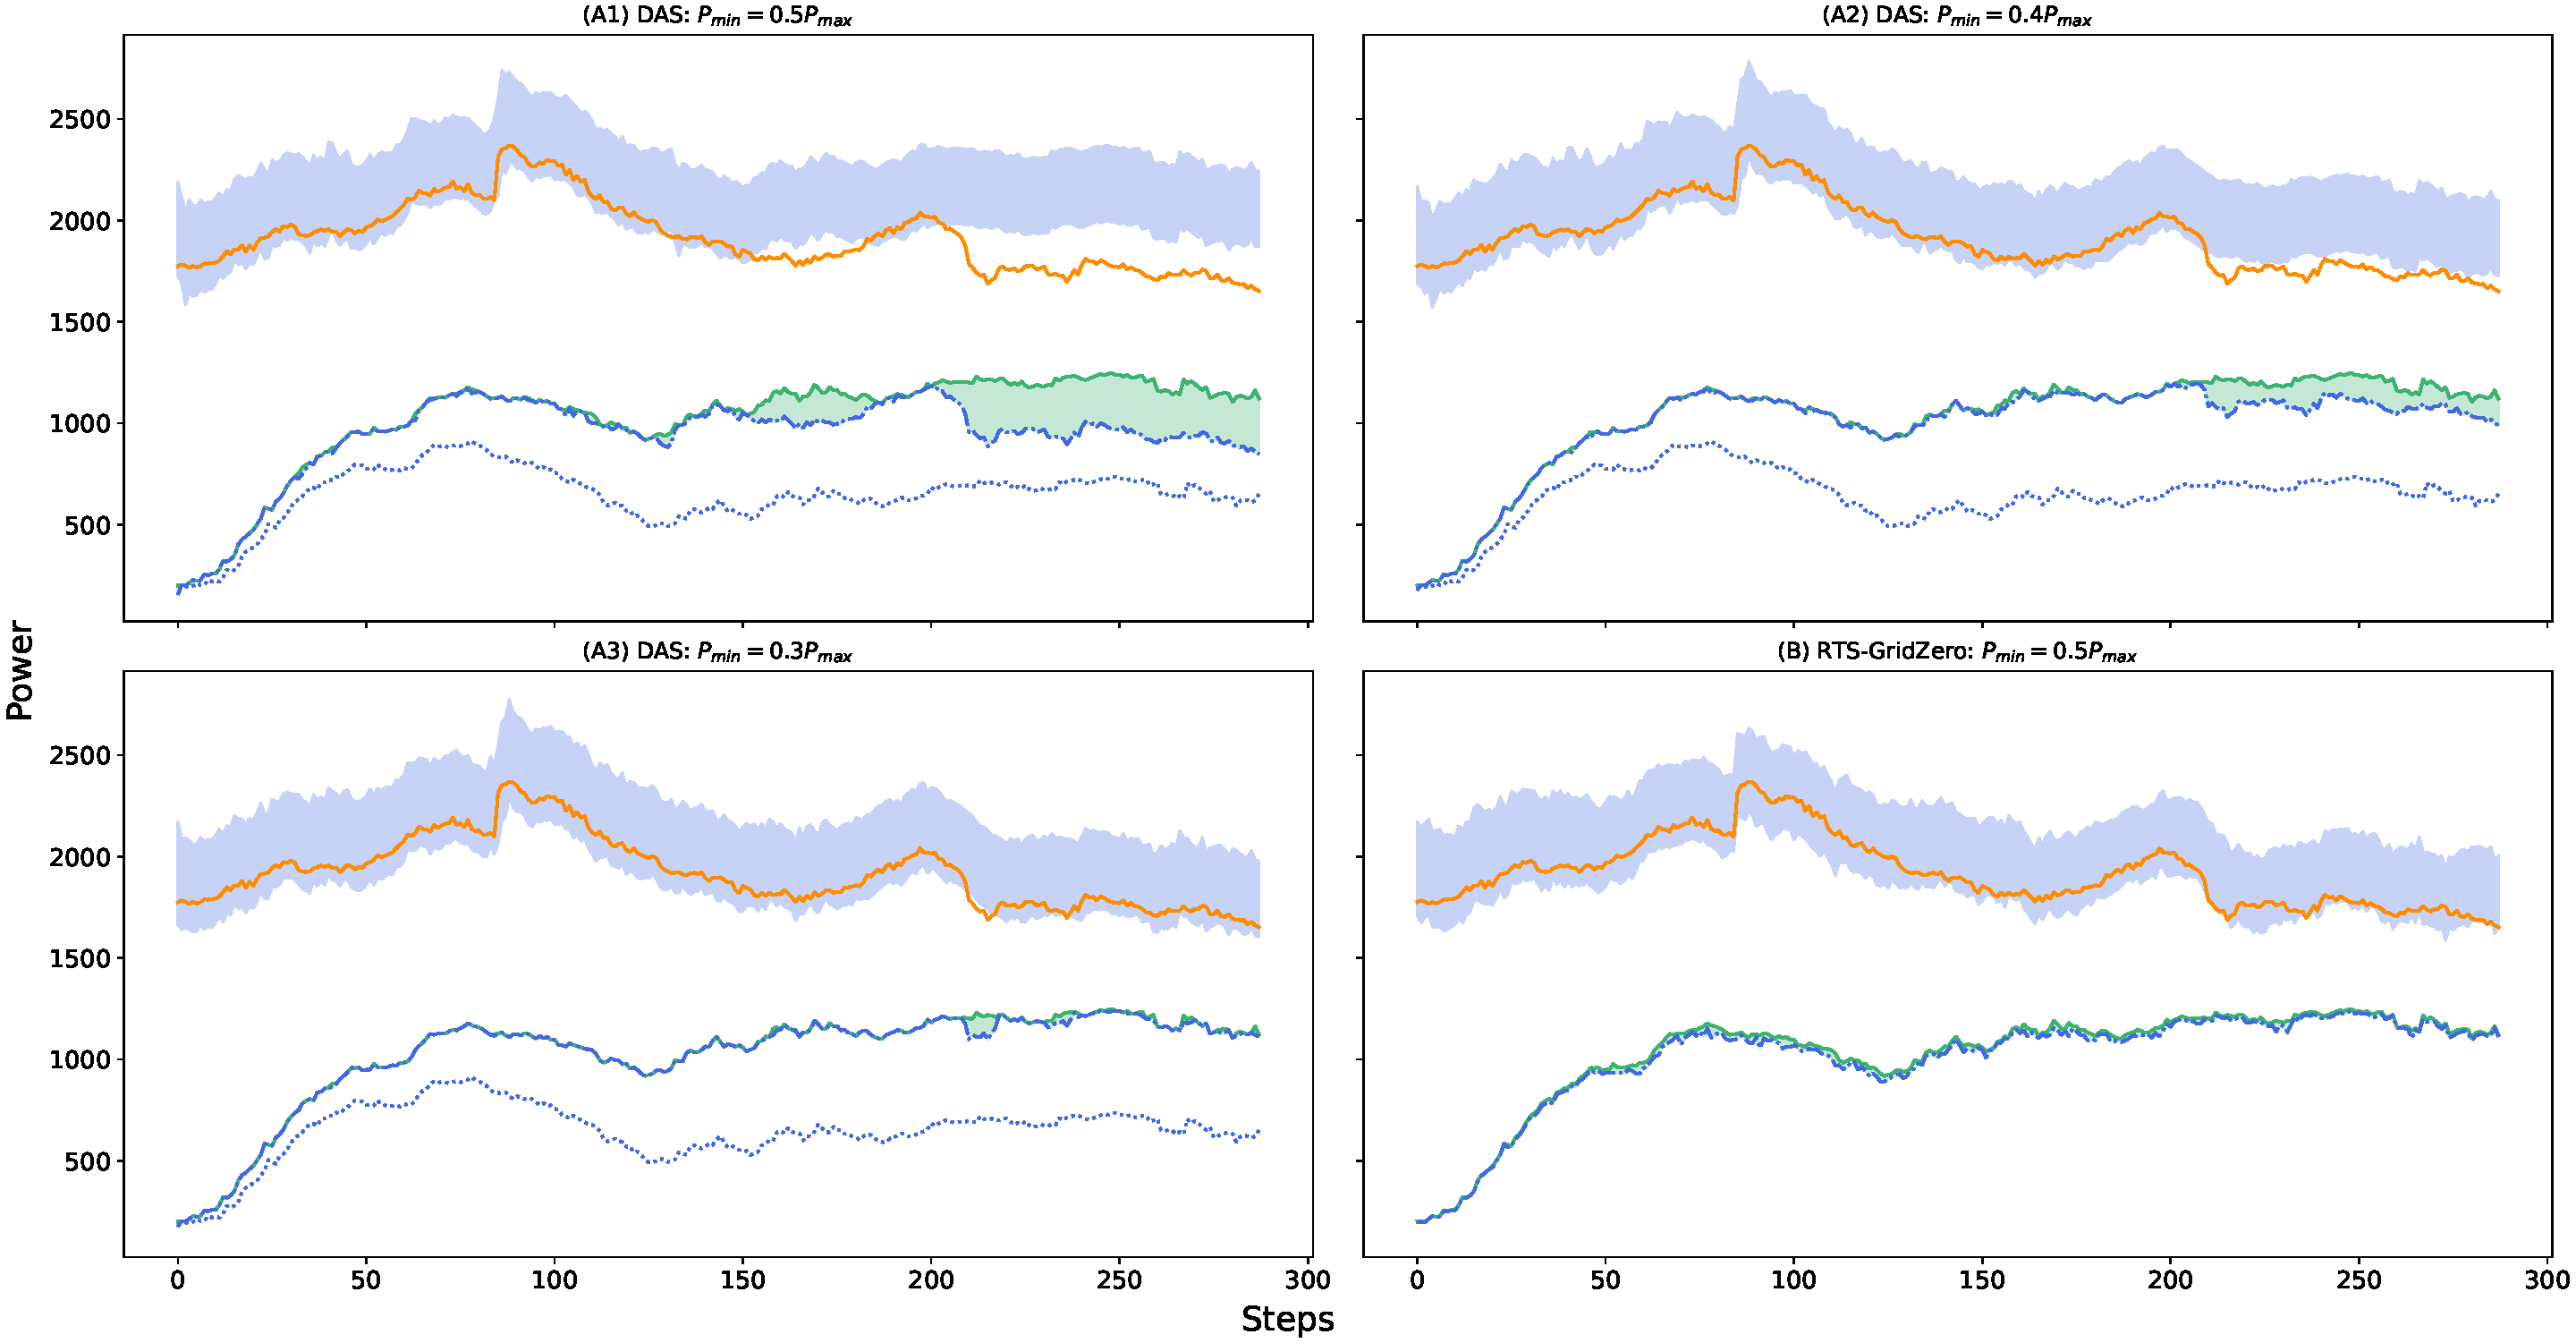
\includegraphics[width=1.0\linewidth]{fig/flexibility_retrofit.pdf}
  \caption{\textbf{Impacts of different flexibility retrofit levels on the scheduling performance.} 
  (A1),(A2) and (A3) shows the flexibility retrofit levels of 
  0\%, 10\% and 20\%, which are corresponding to $\underline{\text{p}}=0.5\,\overline{\text{p}}, 0.4\,\overline{\text{p}}, 0.3\,\overline{\text{p}}$. $\overline{\text{p}}$ and $\underline{\text{p}}$ are the maximum power and minimum power of thermal generators.
  Their results are all based on the DAS. (B) shows the performance of GridZero with $\underline{\text{p}}=0.5\,\overline{\text{p}}$. $\underline{\text{p}}=0.5\,\overline{\text{p}}$ is the most common design of actual thermal generators. $\underline{\text{p}}=0.4\,\overline{\text{p}}$ and $\underline{\text{p}}=0.3\,\overline{\text{p}}$ correspond to 10\% and 20\% flexibility retrofit levels respectively. As we can see, using the DAS approach requires a 20\% flexibility retrofit of conventional thermal units to significantly reduce renewable curtailment. However, the GridZero-based RTS approach achieves the same result without requiring hardware investments to the existing grid through adjusting generators in real-time according to ultra-short-term forecasts.
  } 
  \label{fig:flexibility_retrofit}
\end{figure}

\begin{figure}[h]
    \centering
    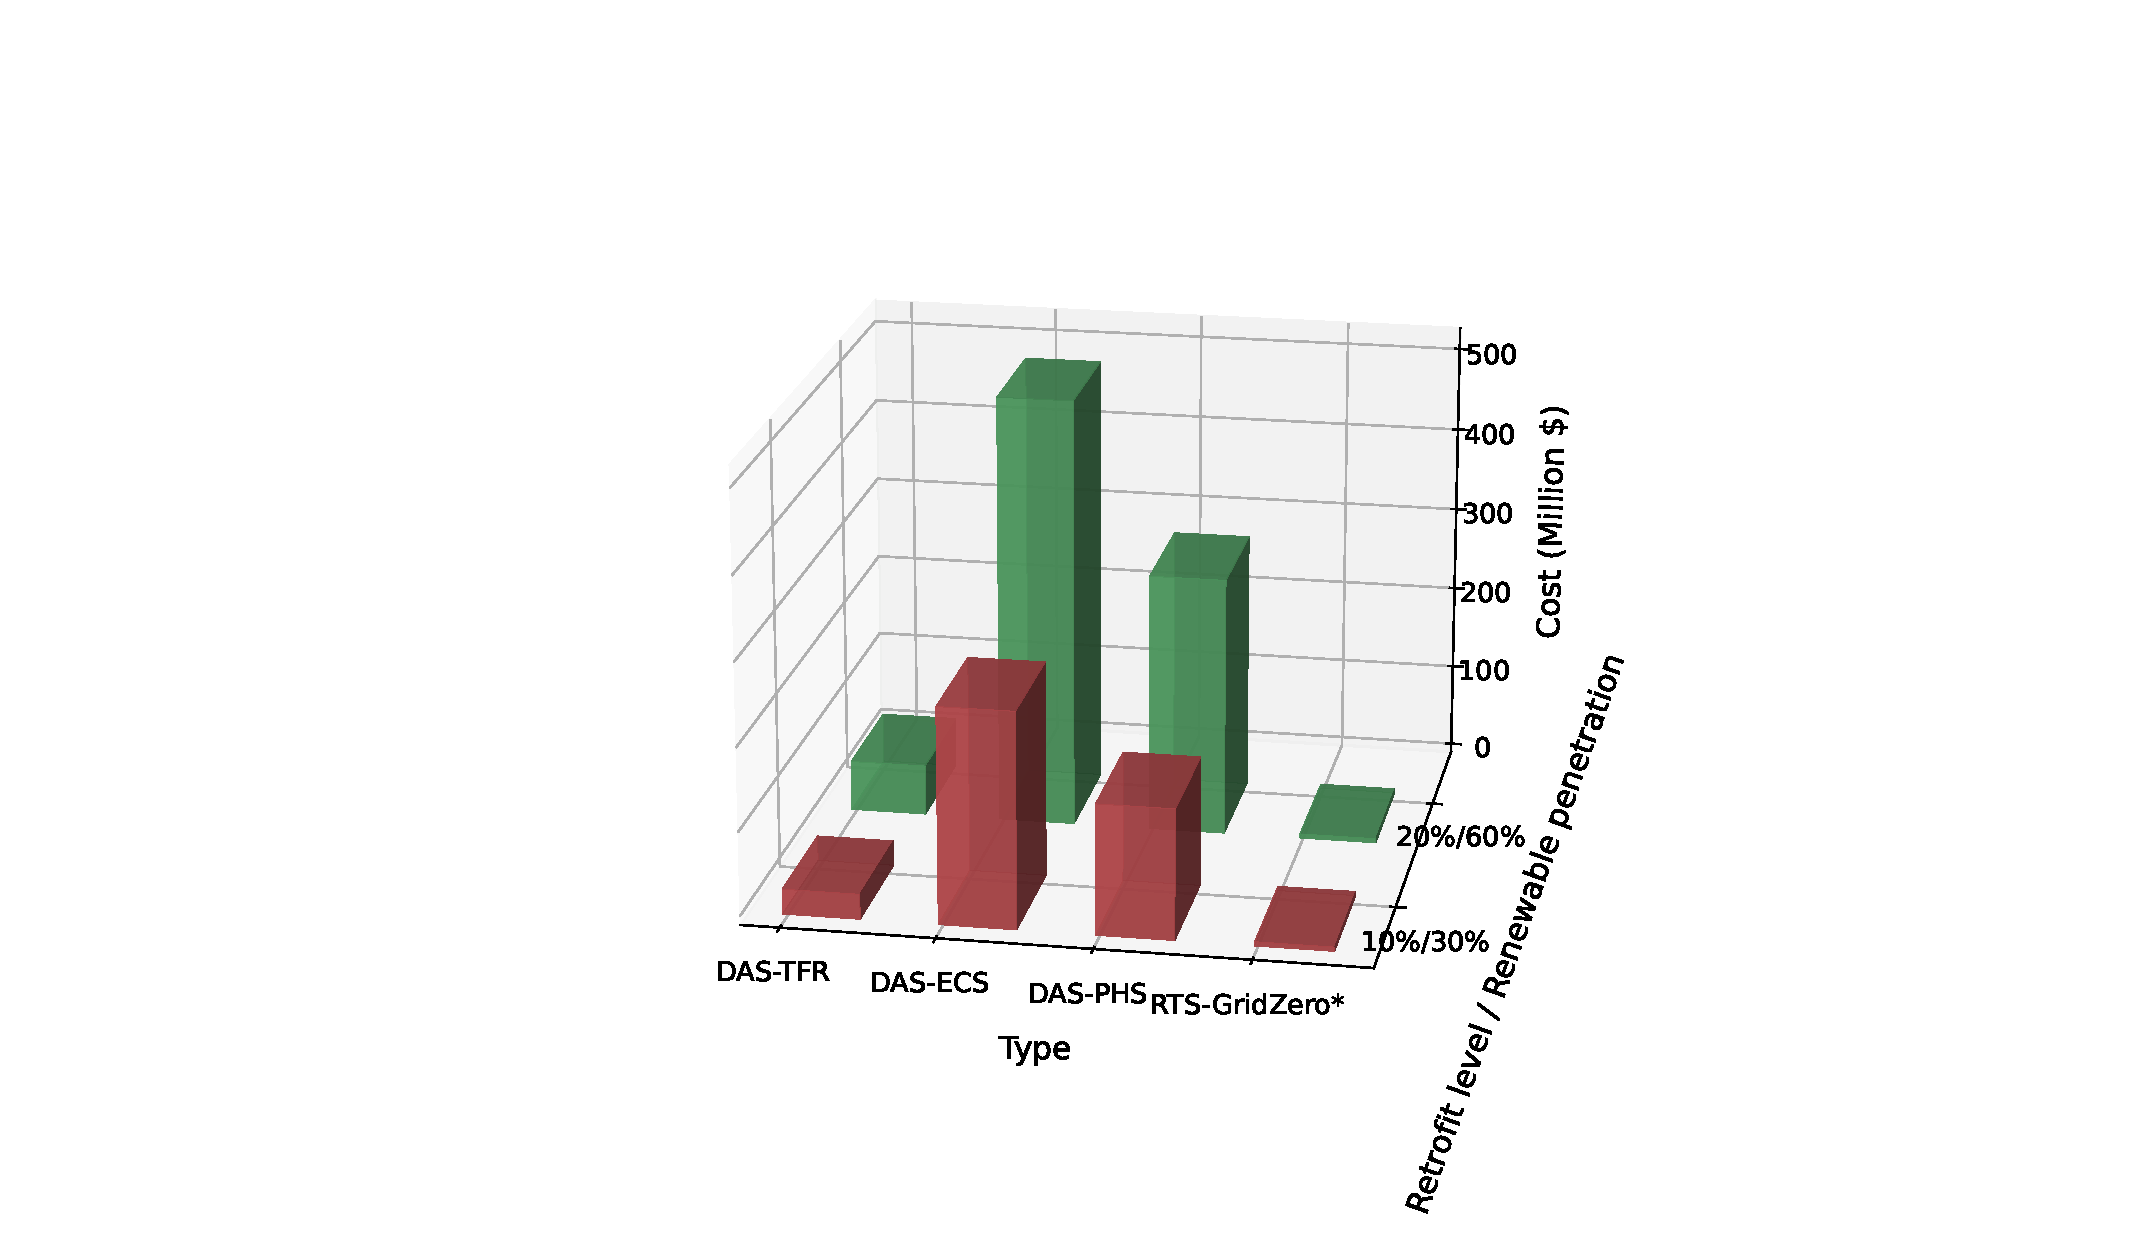
\includegraphics[width=1.0\linewidth]{fig/cost_analysis.pdf}
    \caption{Cost analysis of DAS with hardware upgrades and RTS-GridZero under different levels of renewable energy penetration, in billions of dollars. 
    In the case of renewable energy penetration of 30\%, the capacity of flexibility retrofit or energy storage should reach 10\% of the total installed capacity. While in the case of 60\% penetration, the capacity of flexibility retrofit and energy storage should reach more than 20\%.
    Thermal unit Flexibility Retrofit (TFR) is currently the most cost-effective method, compared with Electro-Chemical Storage (ECS) and Pumped Hydroelectricity Storage (PHS). GridZero simply improves on the scheduling algorithm and does not require additional hardware upgrades, which can save grid operators significant amounts of investments.}
    \label{fig:cost}
\end{figure}

As illustrated in Fig.\ref{fig:flexibility_retrofit}, in order to mitigate renewable curtailment, a retrofit capacity equivalent to 20\% of the total installed capacity is required, which corresponds to 402.2 megawatts of retrofit capacity.
An analysis of China's Jiangxi province indicates that the cost of thermal unit flexibility retrofit is 0.15 million dollars per megawatts~\cite{chen2021flexible}.
Therefore, the total cost of this approach can reach 60.1 million dollars in investment. Additionally, this approach results in the uneconomical operation of thermal units, leading to higher generation costs and increased carbon emissions. According to ~\cite{chen2021flexible}, thermal generators operating at 30\% rated power have 70\% higher cost and 85\% more carbon emission per unit of power generation, compared to those operating at 50\% rated power.

Energy storage is even more expensive than thermal units' flexibility retrofits. The lithium-ion battery is the most cost-effective electrochemical storage choice, but its cost per megawatts is 1.28 million dollars, which is much higher than thermal generator flexibility retrofits~\cite{yan2022lcos}. Although hydro-pumped storage is cheaper than batteries, costing 0.77 million dollars per megawatts~\cite{sospiro2021cost}, 
this physically based long-timescale storage method is still faced with challenges, such as the difficulty of site selection and long construction cycles. As indicated in Fig.\ref{fig:cost}, the cost of constructing energy storage is much higher than the cost of thermal units' flexibility retrofit, despite the same retrofitted level.

In light of these considerations, we investigate the efficacy of our approach in reducing the grid's dependence on energy storage and flexibility retrofits. Fig.\ref{fig:flexibility_retrofit} illustrates that GridZero can achieve a performance level comparable to that of the DAS operating with 20\% retrofitted capacity.
Notably, as Fig.\ref{fig:cost} summarizes, GridZero does not require thermal units' flexibility retrofits or energy storage construction, even if the proportion of renewable energy power generation increases to 60\%. Our methodology relies solely on ultra-short-term forecasts and fast adjustments to enhance dispatch flexibility, which can translate into substantial cost savings for grid construction.
